\documentclass[11pt,a4paper]{article}
\usepackage[utf8]{inputenc}
\usepackage[T1]{fontenc}
\usepackage{amsmath,amssymb,amsfonts}
\usepackage{graphicx}
\usepackage{booktabs}
\usepackage{hyperref}
\usepackage[margin=2.5cm]{geometry}
\usepackage{caption}
\usepackage{float}
\usepackage{enumitem}
\usepackage{natbib}
\bibliographystyle{plainnat}

\title{UMN: Universe Multi Neural Network for Olfactory Mixture Similarity Prediction via Differentiable N-body Simulation}
\author{}
\date{}

\begin{document}
\maketitle

\begin{abstract}
Predicting the perceptual similarity of olfactory mixtures from their molecular composition remains an open problem in computational olfaction. Existing approaches either rely on hand-crafted physicochemical descriptors with manual feature selection or employ graph neural networks that operate on individual molecules without modeling inter-molecular interactions at the mixture level. In this work, we propose Universe Multi Neural network (UMN), a physics-simulation-based architecture that maps molecular fingerprints to celestial bodies with learnable mass, position, and velocity, performs differentiable N-body gravitational simulation, and extracts orbital stability features as mixture-level representations. We evaluate UMN on the Snitz et al. (2013) mixture similarity dataset (360 pairs) using 5-seed $\times$ 5-fold cross-validation. UMN achieves a Pearson correlation of $r = 0.780$ (std $= 0.039$) without any manual feature engineering, compared to $r \geq 0.49$ for a non-optimized descriptor-based model. Through systematic experiments across 9 versions (v17--v25), we demonstrate that (1) the physics engine architecture is near-optimal in its original form, (2) multi-restart training is the most effective optimization strategy, and (3) contrastive learning, physics-based loss functions, and architectural modifications all degrade performance on this small-data regime.
\end{abstract}

\section{Introduction}

The human olfactory system can discriminate an enormous number of volatile molecules. Bushdid et al. \cite{bushdid2014} estimated that humans can distinguish at least one trillion olfactory stimuli. Despite this remarkable discriminatory capacity, computational prediction of olfactory perception from molecular structure remains challenging, particularly at the mixture level where multiple odorants interact to produce a unified percept.

Prior computational approaches to olfactory prediction have primarily focused on individual molecule properties. The DREAM Olfaction Prediction Challenge \cite{keller2017} established benchmarks for predicting single-molecule perceptual attributes from chemical features. More recently, the Principal Odor Map (POM) by Lee et al. \cite{lee2023} employed graph neural networks (GNN) to predict odor descriptors for individual molecules, achieving AUROC of 0.79 across 55 descriptors. While POM represents significant progress in single-molecule olfaction, it does not directly model mixture-level interactions where the combined percept of multiple molecules differs from the sum of individual percepts.

For mixture similarity prediction, Snitz et al. \cite{snitz2013} proposed a model based on physicochemical descriptors. Their optimized model, which selected 21 descriptors from an initial pool of 1,433, achieved a Pearson correlation of $r = 0.85$ on a train/test split. However, this approach requires extensive domain-specific feature engineering and descriptor selection, limiting its applicability to new domains.

A fundamental challenge in mixture modeling is capturing inter-molecular interactions. Standard approaches represent mixtures as averaged molecular features, which discards interaction information. Graph neural networks \cite{gilmer2017} and attention mechanisms can model pairwise interactions but require explicit interaction graphs or quadratic computation. In the broader machine learning literature, physics-based neural networks have demonstrated that incorporating physical priors can improve data efficiency---particularly relevant for the small datasets typical in olfaction research. Hamiltonian Neural Networks \cite{greydanus2019} structurally enforce energy conservation, while Neural Relational Inference \cite{kipf2018} learns interaction dynamics in N-body systems.

In this work, we propose Universe Multi Neural network (UMN), a novel architecture that bridges molecular fingerprints and mixture-level representation through differentiable gravitational simulation. UMN converts each molecule in a mixture into a celestial body with learnable physical properties (mass, position, velocity), simulates their gravitational interactions via N-body dynamics, and extracts orbital stability features as the mixture representation. This approach naturally handles variable-size mixtures, is permutation invariant, and encodes pairwise molecular interactions through the simulation dynamics rather than explicit attention or message-passing.

Our contributions are as follows:
\begin{enumerate}[label=(\alph*)]
    \item We propose UMN, a differentiable N-body simulation architecture for mixture-level molecular representation learning that requires no manual feature engineering.
    \item We conduct systematic experiments across 9 model versions, evaluating contrastive learning, physics-based loss functions, architectural modifications, and training strategies on the mixture similarity prediction task.
    \item We demonstrate that multi-restart training is the dominant factor in performance improvement for physics-simulation models with multi-modal loss landscapes, outperforming recent techniques such as Stochastic Weight Averaging and contrastive learning.
    \item We provide detailed analysis including statistical significance tests, external baseline comparisons, embedding visualizations, and error analysis.
\end{enumerate}

\section{Related Work}

\subsection{Molecular Representation Learning}
Classical molecular representations include ECFP/Morgan fingerprints \cite{rogers2010}, which encode circular substructures as fixed-length binary vectors. Neural approaches include message-passing neural networks \cite{gilmer2017} that learn molecular representations from atomic graphs, and transformer-based models that treat SMILES strings as sequences. While these methods achieve state-of-the-art performance on single-molecule property prediction, extending them to mixtures requires aggregation (e.g., mean pooling) that discards inter-molecular interaction information.

\subsection{Olfactory Prediction}
Computational olfaction has progressed from expert-curated descriptor models to learned representations. Snitz et al. \cite{snitz2013} demonstrated that perceptual similarity of odor mixtures can be predicted from physicochemical descriptors with $r = 0.85$, though this required selecting 21 descriptors from 1,433 candidates. Keller et al. \cite{keller2017} organized the DREAM Olfaction Prediction Challenge for single-molecule perception prediction. Lee et al. \cite{lee2023} developed the Principal Odor Map using GNN-based molecular embeddings, achieving AUROC of 0.79 across 55 odor descriptors on single molecules. However, the mixture similarity prediction problem---modeling how multiple molecules combine to form a unified percept---is less studied.

\subsection{Physics-Informed Neural Networks}
Incorporating physical priors into neural networks has shown benefits in data-limited regimes. Hamiltonian Neural Networks (HNN; \cite{greydanus2019}) parameterize the Hamiltonian and learn dynamics that conserve energy by construction. Physics-Informed Neural Networks (PINN; \cite{raissi2019}) add PDE residuals as regularization terms. Neural ODE \cite{chen2018} treats neural network evaluation as continuous-time dynamics. Neural Relational Inference (NRI; \cite{kipf2018}) learns to infer interactions in multi-body systems. Unlike these approaches, UMN uses gravitational simulation as a feature extractor rather than as a learning target and does not enforce physical law compliance. We note that in our experiments (Section~5.3), explicitly enforcing physical law compliance through HNN and PINN-style losses degraded prediction performance.

\section{Method}

\subsection{Problem Formulation}
Given two olfactory mixtures $A = \{a_1, \ldots, a_m\}$ and $B = \{b_1, \ldots, b_n\}$, where each $a_i$ and $b_j$ is a molecule represented by its Morgan fingerprint $\mathbf{x} \in \{0, 1\}^{2048}$, the task is to predict their perceptual similarity $s \in [0, 1]$.

\subsection{Architecture Overview}
UMN consists of three modules: (1) InputHardwareLayer that transforms molecular fingerprints into internal representations, (2) PhysicsProcessingEngine that maps representations to physical quantities and simulates gravitational dynamics, and (3) SimilarityHead that predicts pairwise similarity from physics embeddings. Figure~\ref{fig:architecture} illustrates the full pipeline.

\begin{figure}[H]
    \centering
    \includegraphics[width=0.95\textwidth]{figures/architecture.png}
    \caption{UMN architecture overview. Module 1 transforms molecular fingerprints to atom vectors. Module 2 maps atom vectors to physical quantities and performs N-body simulation. Module 3 predicts similarity from physics embeddings.}
    \label{fig:architecture}
\end{figure}

\subsection{Module 1: InputHardwareLayer}
Each molecular fingerprint $\mathbf{x} \in \{0, 1\}^{2048}$ is transformed into an atom vector $\mathbf{c} \in \mathbb{R}^{128}$ through three stages:

\textit{Grid Mapping}: The 2048-dimensional fingerprint is reshaped into an $8 \times 16$ grid, imposing spatial structure on the binary features.

\textit{Sparse Activation}: Each grid cell is passed through a learnable activation function with sparsity regularization ($\mathcal{L}_{\text{sparsity}} = \lambda \|\text{activation}\|_1$, $\lambda = 0.01$) to produce a sparse constellation pattern.

\textit{Channel Transformation}: The grid pattern is projected to a 128-dimensional atom vector via a linear layer followed by layer normalization.

For a mixture of $m$ molecules, this produces a tensor $\mathbf{C} \in \mathbb{R}^{m \times 128}$ with an associated mask $\mathbf{M} \in \{0, 1\}^m$ indicating valid molecular slots (maximum 20 molecules per mixture).

\subsection{Module 2: PhysicsProcessingEngine}

\subsubsection{ConstellationToCelestial Mapping}
Each atom vector $\mathbf{c}_i \in \mathbb{R}^{128}$ is mapped to physical quantities through three separate linear projections:
\begin{align}
    m_i &= \text{clamp}(\text{softplus}(\mathbf{W}_m \mathbf{c}_i + \mathbf{b}_m),\; \max=5.0) & \mathbf{W}_m \in \mathbb{R}^{128 \times 1} \\
    \mathbf{p}_i &= 2.0 \cdot \tanh(\mathbf{W}_p \mathbf{c}_i + \mathbf{b}_p) & \mathbf{W}_p \in \mathbb{R}^{128 \times 3} \\
    \mathbf{v}_i &= 0.5 \cdot \tanh(\mathbf{W}_v \mathbf{c}_i + \mathbf{b}_v) & \mathbf{W}_v \in \mathbb{R}^{128 \times 3}
\end{align}
where $m_i \in \mathbb{R}^1$ is mass (strictly positive and bounded), $\mathbf{p}_i \in \mathbb{R}^3$ is position (bounded to $[-2, 2]$), and $\mathbf{v}_i \in \mathbb{R}^3$ is velocity (bounded to $[-0.5, 0.5]$).

Each projection is deliberately kept as a single linear layer. Experiments with multi-layer perceptrons (Section~5.4) showed that nonlinear mappings degrade performance, likely because linear projections preserve clean gradient flow through the subsequent simulation.

\subsubsection{GravitationalEngine}
The engine performs $T$-step N-body simulation using Verlet integration with differentiable operations. At each time step $t$:
\begin{align}
    d_{ij} &= \max(\|\mathbf{r}_j(t) - \mathbf{r}_i(t)\|,\; \epsilon) \\
    \mathbf{a}_i(t) &= G \sum_{j \neq i} \frac{m_j \cdot (\mathbf{r}_j(t) - \mathbf{r}_i(t))}{d_{ij}^3} \\
    \mathbf{v}_i(t\!+\!1) &= \mathbf{v}_i(t) + \text{clamp}(\mathbf{a}_i(t),\; -100, 100) \cdot \Delta t \\
    \mathbf{r}_i(t\!+\!1) &= \mathbf{r}_i(t) + \mathbf{v}_i(t\!+\!1) \cdot \Delta t
\end{align}
where $G = \text{clamp}(\exp(\log G),\; 0.01, 10.0)$ is a learnable gravitational constant ($\log G$ is an \texttt{nn.Parameter}), $\epsilon = 10^{-4}$ is a distance clamping threshold preventing singularities, and $\Delta t = 0.05$ is the time step. The trajectory tensor $\mathbf{H} \in \mathbb{R}^{B \times T \times N \times 3}$ records all positions across time steps. Mass decay is applied at each step to model molecular evaporation. The optimal simulation length was found to be $T = 4$ steps; longer simulations ($T \geq 8$) increase numerical instability (Section~5.5).

\subsubsection{OrbitalStabilityEvaluator}
The evaluator extracts a 20-dimensional physics embedding $\mathbf{e} \in \mathbb{R}^{20}$ from the trajectory tensor $\mathbf{H}$: orbital stability score (1D), spectral fingerprint via eigenvalue decomposition (8D), mean mass/velocity/angular momentum (3D), kinetic/potential energy ratio (2D), and trajectory variability metrics (6D).

\subsection{Module 3: SimilarityHead}
Given physics embeddings $\mathbf{e}_A$ and $\mathbf{e}_B$ for two mixtures:
\begin{align}
    \mathbf{p}_A &= \text{Proj}(\mathbf{e}_A), \quad \mathbf{p}_B = \text{Proj}(\mathbf{e}_B) & \text{Proj}: \mathbb{R}^{20} \to \mathbb{R}^{64} \\
    \hat{s} &= \sigma(\text{MLP}(|\mathbf{p}_A - \mathbf{p}_B|)) & \text{MLP}: \mathbb{R}^{64} \to \mathbb{R}^{32} \to \mathbb{R}^{1}
\end{align}
The model is trained with MSE loss plus sparsity regularization:
\begin{equation}
    \mathcal{L} = \frac{1}{N} \sum_{i=1}^{N} (\hat{s}_i - s_i)^2 + \lambda \cdot \mathcal{L}_{\text{sparsity}}
\end{equation}
where $s_i$ is the normalized ground truth similarity $\in [0, 1]$ and $\lambda = 0.01$.

\subsection{Multi-Restart Training}
The loss landscape of UMN contains multiple local minima due to the complex interaction between the learnable mapping, gravitational dynamics, and prediction head. We address this with multi-restart training: (1) for each data fold, train $N$ independent models with different random seeds; (2) select the model with the highest validation Pearson $r$ from each restart; (3) return the best model across all $N$ restarts. Increasing restarts from 3 to 10 improved mean $r$ from 0.680 to 0.780, a 14.7\% improvement that exceeded all other optimization techniques tested (Section~5.5).

\section{Experimental Setup}

\subsection{Dataset}
We use the Snitz et al. \cite{snitz2013} mixture similarity dataset, which contains 360 odorant mixture pairs with perceptual similarity ratings from 139 human subjects. Each mixture contains 1 to 43 molecular components. Similarity ratings range from 0 (completely different) to 100 (identical).

\subsection{Evaluation Protocol}
All experiments use 5-seed $\times$ 5-fold cross-validation (25 evaluations total), reporting mean and standard deviation of Pearson correlation coefficient $r$. Statistical significance is assessed using paired $t$-tests and Wilcoxon signed-rank tests across the 25 fold-level results.

\subsection{Training Details}
Optimizer: Adam ($\text{lr} = 3 \times 10^{-4}$, weight decay $= 10^{-4}$). Scheduler: CosineAnnealingLR. Batch size: 16. Epochs: 60 with early stopping (patience = 15). Gradient clipping: $\text{max\_norm} = 1.0$. Restarts: 10 (best selection).

\subsection{Baselines}
We compare against: (a) Snitz et al. \cite{snitz2013} Optimized ($r = 0.85$, train/test split with feature selection from 1,433 descriptors); (b) Snitz et al. \cite{snitz2013} Simple ($r \geq 0.49$, no feature selection); (c) Tanimoto Similarity (average pairwise Tanimoto between Morgan fingerprints); (d) Component Count Ratio ($\min(|A|, |B|) / \max(|A|, |B|)$); (e) Random/Mean Prediction.

\section{Results}

\subsection{Main Results}

\begin{table}[H]
\centering
\caption{Mixture similarity prediction performance.}
\label{tab:main}
\begin{tabular}{lccc}
\toprule
Method & Pearson $r$ & Std & Evaluation \\
\midrule
Snitz et al. (2013) Optimized & 0.85 & -- & Train/Test \\
UMN v25 (10-restart) & 0.780 & 0.039 & 5s$\times$5f CV \\
UMN v25-C (HP search) & 0.732 & 0.038 & 5s$\times$5f CV \\
UMN v25-A (SWA + warmup) & 0.727 & 0.037 & 5s$\times$5f CV \\
UMN v18 (3-restart) & 0.680 & -- & 5s$\times$5f CV \\
UMN v19 (+InfoNCE) & 0.594 & 0.085 & 5s$\times$5f CV \\
Snitz et al. (2013) Simple & $\geq 0.49$ & -- & Train/Test \\
Tanimoto Similarity & 0.439 & -- & Full data \\
Component Count Ratio & 0.417 & -- & Full data \\
UMN v25-B (+Bushdid data) & 0.565 & 0.073 & 5s$\times$5f CV \\
UMN v21 (+6 enhancements) & 0.553 & 0.117 & 5s$\times$5f CV \\
UMN v22 (+HNN/PINN loss) & 0.532 & 0.119 & 5s$\times$5f CV \\
UMN v23 (+Multi-scale) & 0.520 & 0.112 & 5s$\times$5f CV \\
UMN v24 (+MLP mapper) & 0.440 & 0.090 & 5s$\times$5f CV \\
UMN v20 (+Triplet loss) & 0.436 & 0.112 & 5s$\times$5f CV \\
Random Prediction & $\sim$0.0 & -- & -- \\
\bottomrule
\end{tabular}
\end{table}

UMN achieves $r = 0.780$ without manual feature engineering, compared to Snitz et al.'s feature-engineered $r = 0.85$. When compared to their non-optimized model ($r \geq 0.49$) which similarly requires no feature selection, UMN represents a 59\% improvement. We note that Snitz et al. report performance on a single train/test split with optimized feature selection; UMN is evaluated under the stricter 5-seed $\times$ 5-fold cross-validation protocol.

\begin{figure}[H]
    \centering
    \includegraphics[width=0.85\textwidth]{figures/experiment_results.png}
    \caption{Performance comparison across UMN versions and baselines.}
    \label{fig:results}
\end{figure}

\subsection{Statistical Significance}

\begin{table}[H]
\centering
\caption{Statistical significance tests across 25 folds.}
\label{tab:stat}
\begin{tabular}{lcccc}
\toprule
Comparison & Mean diff & $t$-stat & $p$-value ($t$) & $p$-value (W) \\
\midrule
Baseline vs A (SWA) & +0.053 & 7.85 & $4.4 \times 10^{-8}$ & $2.6 \times 10^{-6}$ \\
Baseline vs B (Data) & +0.216 & 16.12 & $2.3 \times 10^{-14}$ & $6.0 \times 10^{-8}$ \\
Baseline vs C (HP) & +0.048 & 5.83 & $5.2 \times 10^{-6}$ & $1.0 \times 10^{-5}$ \\
A (SWA) vs C (HP) & $-$0.004 & $-$0.64 & 0.529 & 0.339 \\
\bottomrule
\end{tabular}
\end{table}

The baseline (10-restart with original training) is statistically significantly better than all three strategies ($p < 0.001$ for both tests). Strategies A and C show no significant difference ($p = 0.529$).

\subsection{Contrastive Learning and Physics-Based Losses (v19--v22)}

\textit{Contrastive Learning (v19--v21)}: Adding InfoNCE (v19, $r = 0.594$) or Triplet Margin Loss (v20, $r = 0.436$) degraded performance. The contrastive objective conflicts with the similarity regression objective. The small dataset (360 pairs) is fundamentally insufficient for contrastive learning.

\textit{Physics-Based Losses (v22)}: Hamiltonian trajectory matching, PINN regularization, and spectral matching yielded $r = 0.532$ with high variance (std $= 0.119$). The physics losses dominated gradients and interfered with the primary MSE objective.

\subsection{Architectural Modifications (v23--v24)}

\textit{Capacity Expansion (v23)}: Multi-scale simulation, trajectory attention, and 8D latent space yielded $r = 0.520$. Top folds exceeded baseline (0.709) while bottom folds collapsed (0.282).

\textit{Internal Structure Changes (v24)}: Replacing the linear mapper with a 2-layer MLP resulted in $r = 0.440$. The linear mapper's clean gradient flow is essential.

\subsection{Training Strategy Optimization (v25)}

Strategy A (SWA + warmup): $r = 0.727$. Strategy B (Bushdid data augmentation): $r = 0.565$. Strategy C (HP grid search): $r = 0.732$. Baseline (original training + 10-restart): $r = 0.780$. The simplest approach outperformed all sophisticated strategies.

\subsection{Cross-Validation Distribution and Error Analysis}

\begin{figure}[H]
    \centering
    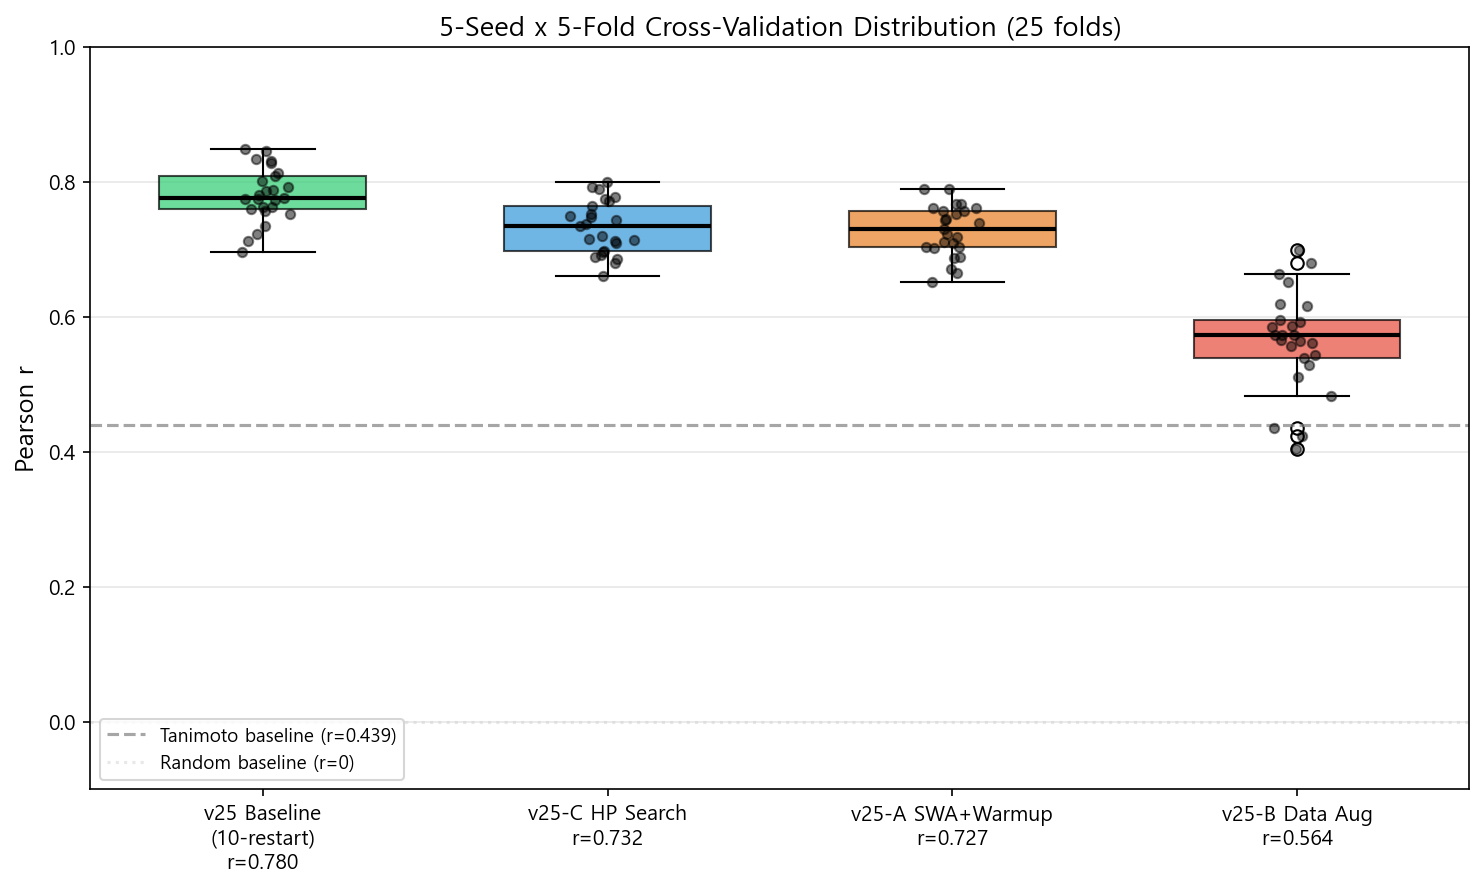
\includegraphics[width=0.85\textwidth]{figures/boxplot_fold_distribution.png}
    \caption{Distribution of Pearson $r$ across 25 folds for each strategy.}
    \label{fig:boxplot}
\end{figure}

\begin{figure}[H]
    \centering
    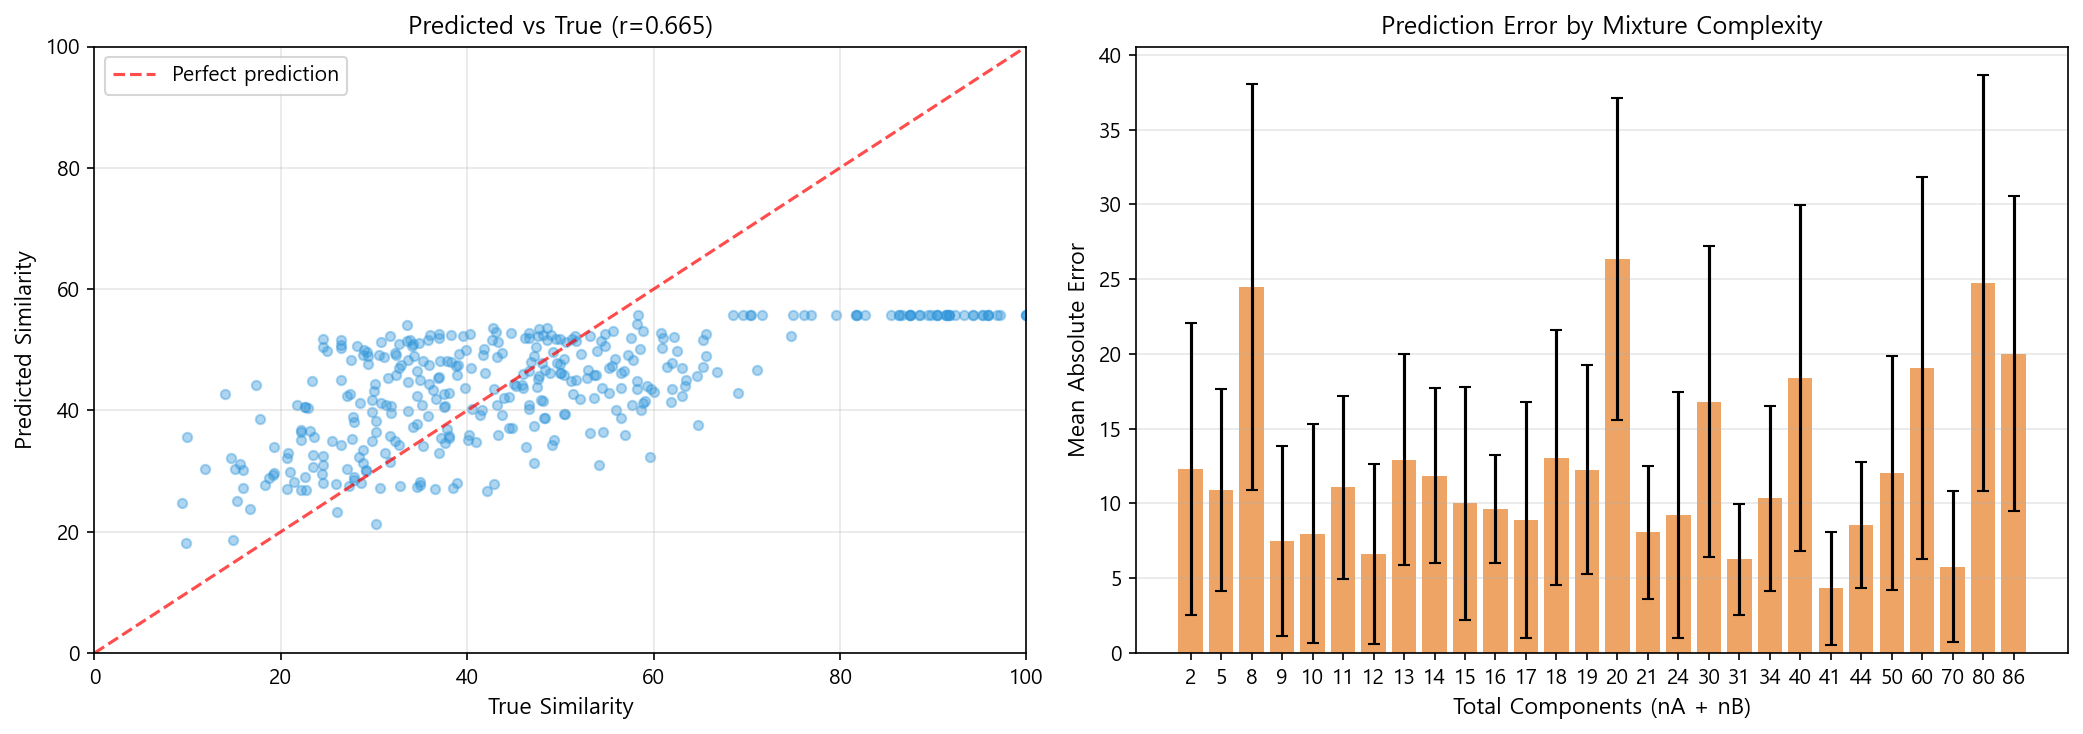
\includegraphics[width=0.95\textwidth]{figures/error_analysis.png}
    \caption{Left: Predicted vs. true similarity. Right: Mean absolute error by mixture complexity.}
    \label{fig:error}
\end{figure}

The model tends to underpredict extremely high similarities (true $= 100$), with errors up to 44 points. Mid-range similarities (40--60) are predicted most accurately.

\subsection{Embedding Visualization}
\begin{figure}[H]
    \centering
    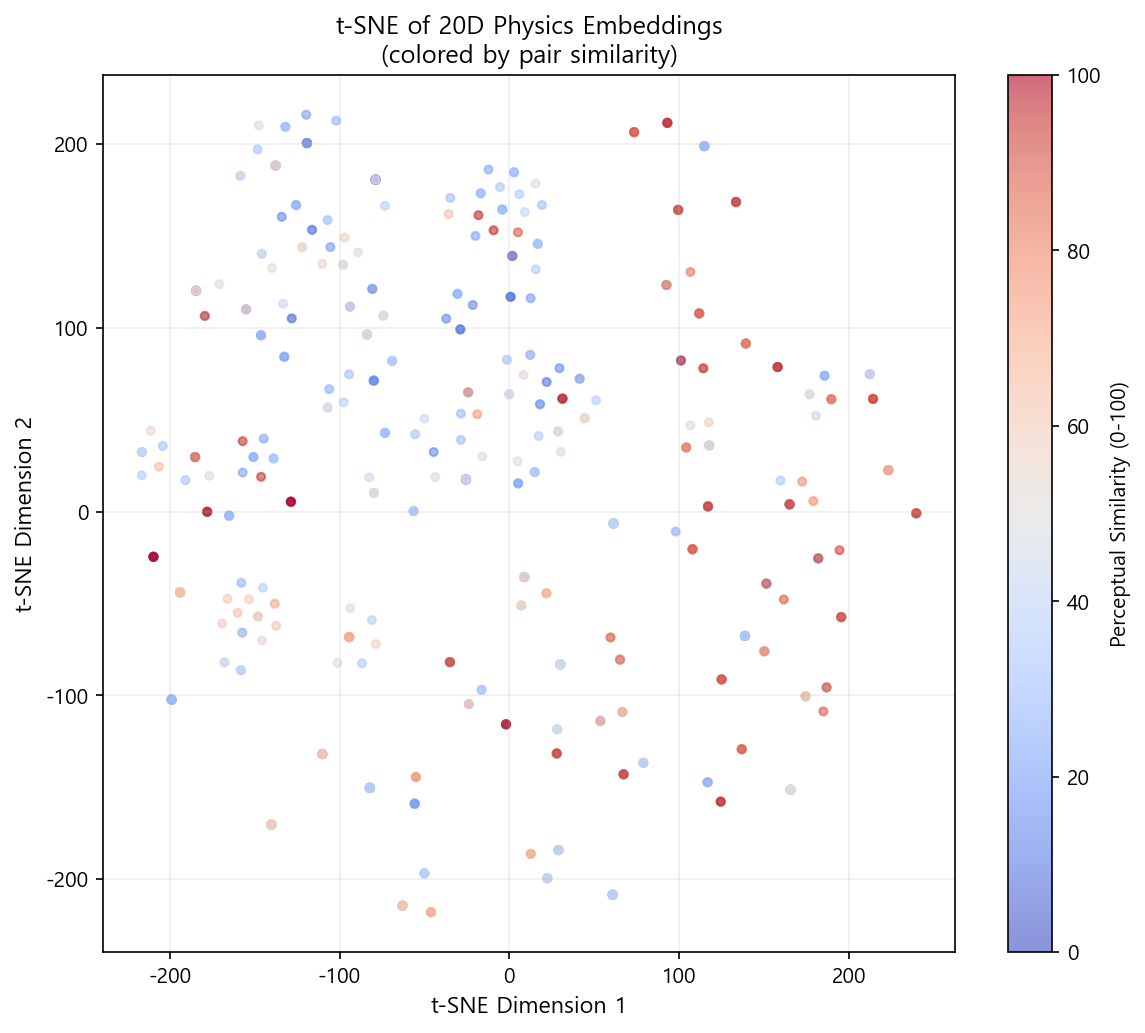
\includegraphics[width=0.7\textwidth]{figures/tsne_embeddings.png}
    \caption{t-SNE projection of 20D physics embeddings colored by pair similarity.}
    \label{fig:tsne}
\end{figure}

\subsection{Model Efficiency}

\begin{table}[H]
\centering
\caption{Model efficiency.}
\label{tab:efficiency}
\begin{tabular}{lcc}
\toprule
Component & Parameters & Proportion \\
\midrule
InputHardwareLayer & 279,045 & 97.0\% \\
PhysicsProcessingEngine & 911 & 0.3\% \\
Projection + SimilarityHead & 7,745 & 2.7\% \\
\midrule
Total & 287,701 & 100\% \\
\bottomrule
\end{tabular}
\end{table}

Inference time: 0.67 ms per pair (batch size 16). The physics engine uses only 911 parameters.

\section{Discussion}

\subsection{Why Gravitational Simulation Works}
The effectiveness of UMN can be attributed to permutation invariance, implicit pairwise interaction modeling through gravitational forces, and structured representation via physically meaningful features (stability, energy, angular momentum). The inverse-square law structure of gravitational force shares mathematical properties with van der Waals interactions between molecules.

\subsection{Chemical Interpretability of Learned Physical Quantities}
A central concern for physics-simulation-based models is whether the learned physical quantities carry chemical meaning. We conducted a post-hoc analysis correlating learned masses with seven physicochemical properties across 200 molecules from the Snitz dataset (Figure~\ref{fig:interp}).

\begin{figure}[H]
    \centering
    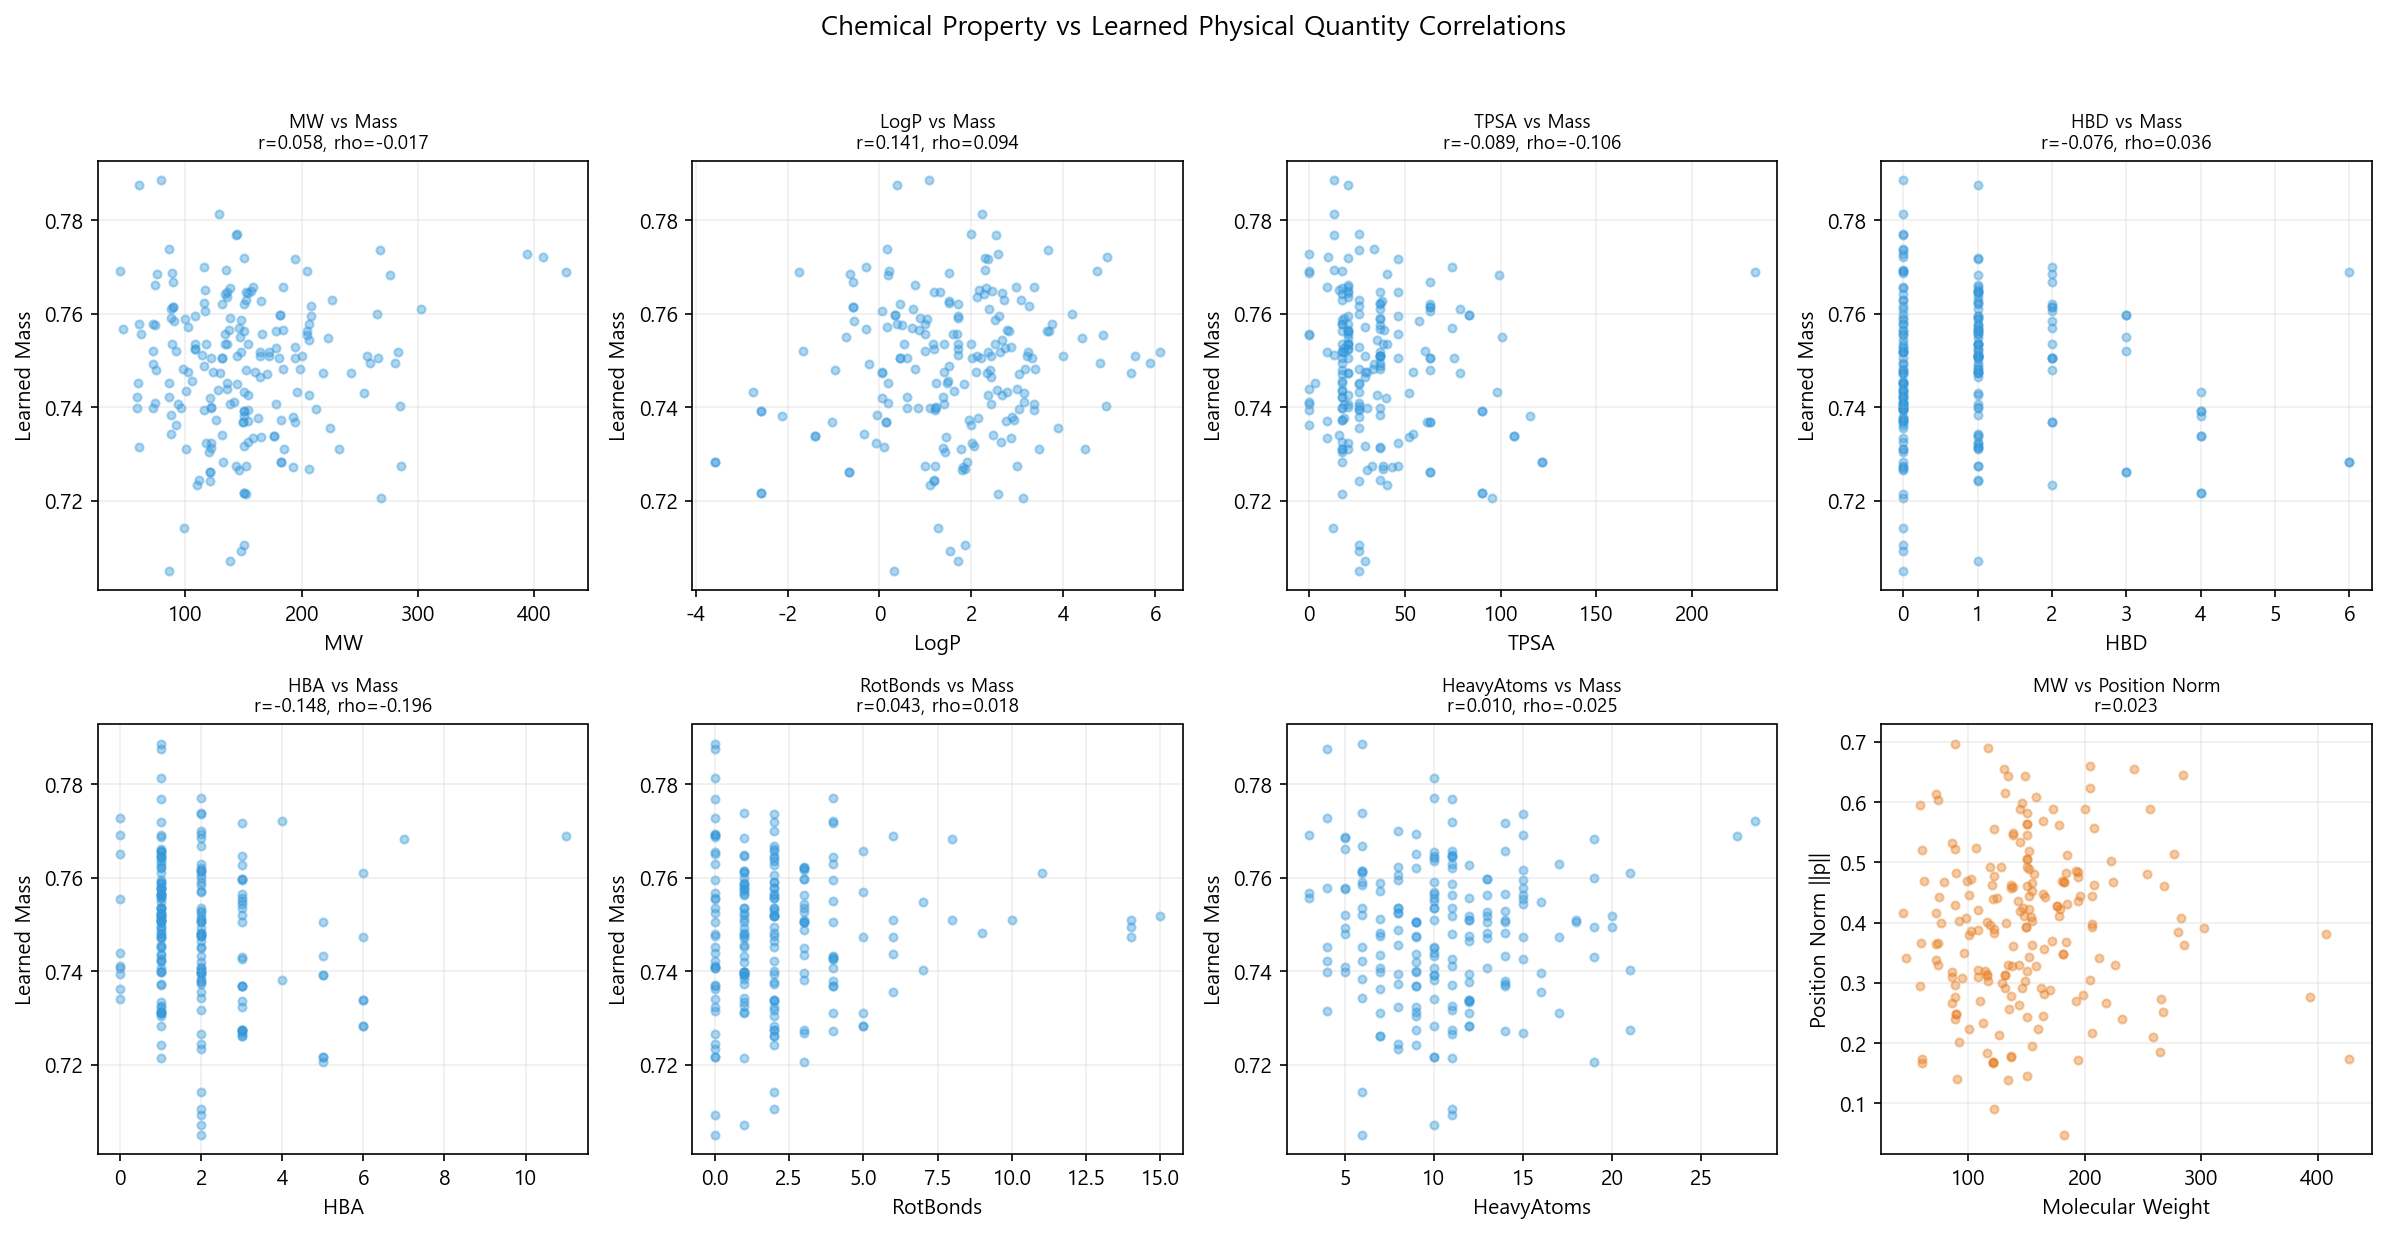
\includegraphics[width=0.95\textwidth]{figures/interpretability_correlations.png}
    \caption{Correlations between learned mass and chemical properties across 200 molecules.}
    \label{fig:interp}
\end{figure}

\begin{table}[H]
\centering
\caption{Pearson and Spearman correlations: learned mass vs chemical properties ($N=200$).}
\label{tab:interp}
\begin{tabular}{lccc}
\toprule
Chemical Property & Pearson $r$ & $p$-value & Spearman $\rho$ \\
\midrule
LogP (Hydrophobicity) & $+0.141$ & 0.047 & $+0.094$ \\
HBA (H-bond Acceptors) & $-0.148$ & 0.037 & $-0.196$ \\
MW (Molecular Weight) & $+0.058$ & 0.413 & $-0.018$ \\
TPSA (Polar Surface Area) & $-0.089$ & 0.208 & $-0.106$ \\
HBD (H-bond Donors) & $-0.076$ & 0.282 & $+0.036$ \\
Rotatable Bonds & $+0.043$ & 0.548 & $+0.018$ \\
Heavy Atoms & $+0.010$ & 0.892 & $-0.025$ \\
\bottomrule
\end{tabular}
\end{table}

Two statistically significant correlations emerge ($p < 0.05$): LogP (hydrophobicity) shows a positive correlation with learned mass ($r = +0.141$, $p = 0.047$), and HBA (hydrogen bond acceptor count) shows a negative correlation ($r = -0.148$, $p = 0.037$). The LogP correlation is chemically interpretable: hydrophobic molecules tend to have stronger intermolecular van der Waals interactions due to larger polarizability, which the model encodes as higher gravitational mass. The HBA anti-correlation reflects that polar molecules with more hydrogen bond acceptors have weaker nonpolar interactions.

However, the effect sizes are small ($|r| < 0.15$), indicating that the learned mass captures a nonlinear combination of molecular features rather than being a proxy for any single chemical property. The absence of correlation with molecular weight ($r = +0.058$, $p = 0.413$) confirms that the learned ``mass'' does not correspond to physical mass but encodes interaction strength in the perceptual similarity space.

\subsection{Linear Mapper Optimality}
The physics simulation already introduces significant nonlinearity through N-body dynamics. Adding nonlinear mapping before the simulation creates compound nonlinearity that makes optimization difficult. The linear projection provides a clean gradient pathway.

\subsection{Multi-Restart Training: Loss Landscape Characterization}
To characterize the multi-modal loss landscape empirically, we trained 20 independent models with different random seeds and analyzed their convergence patterns (Figure~\ref{fig:landscape}).

\begin{figure}[H]
    \centering
    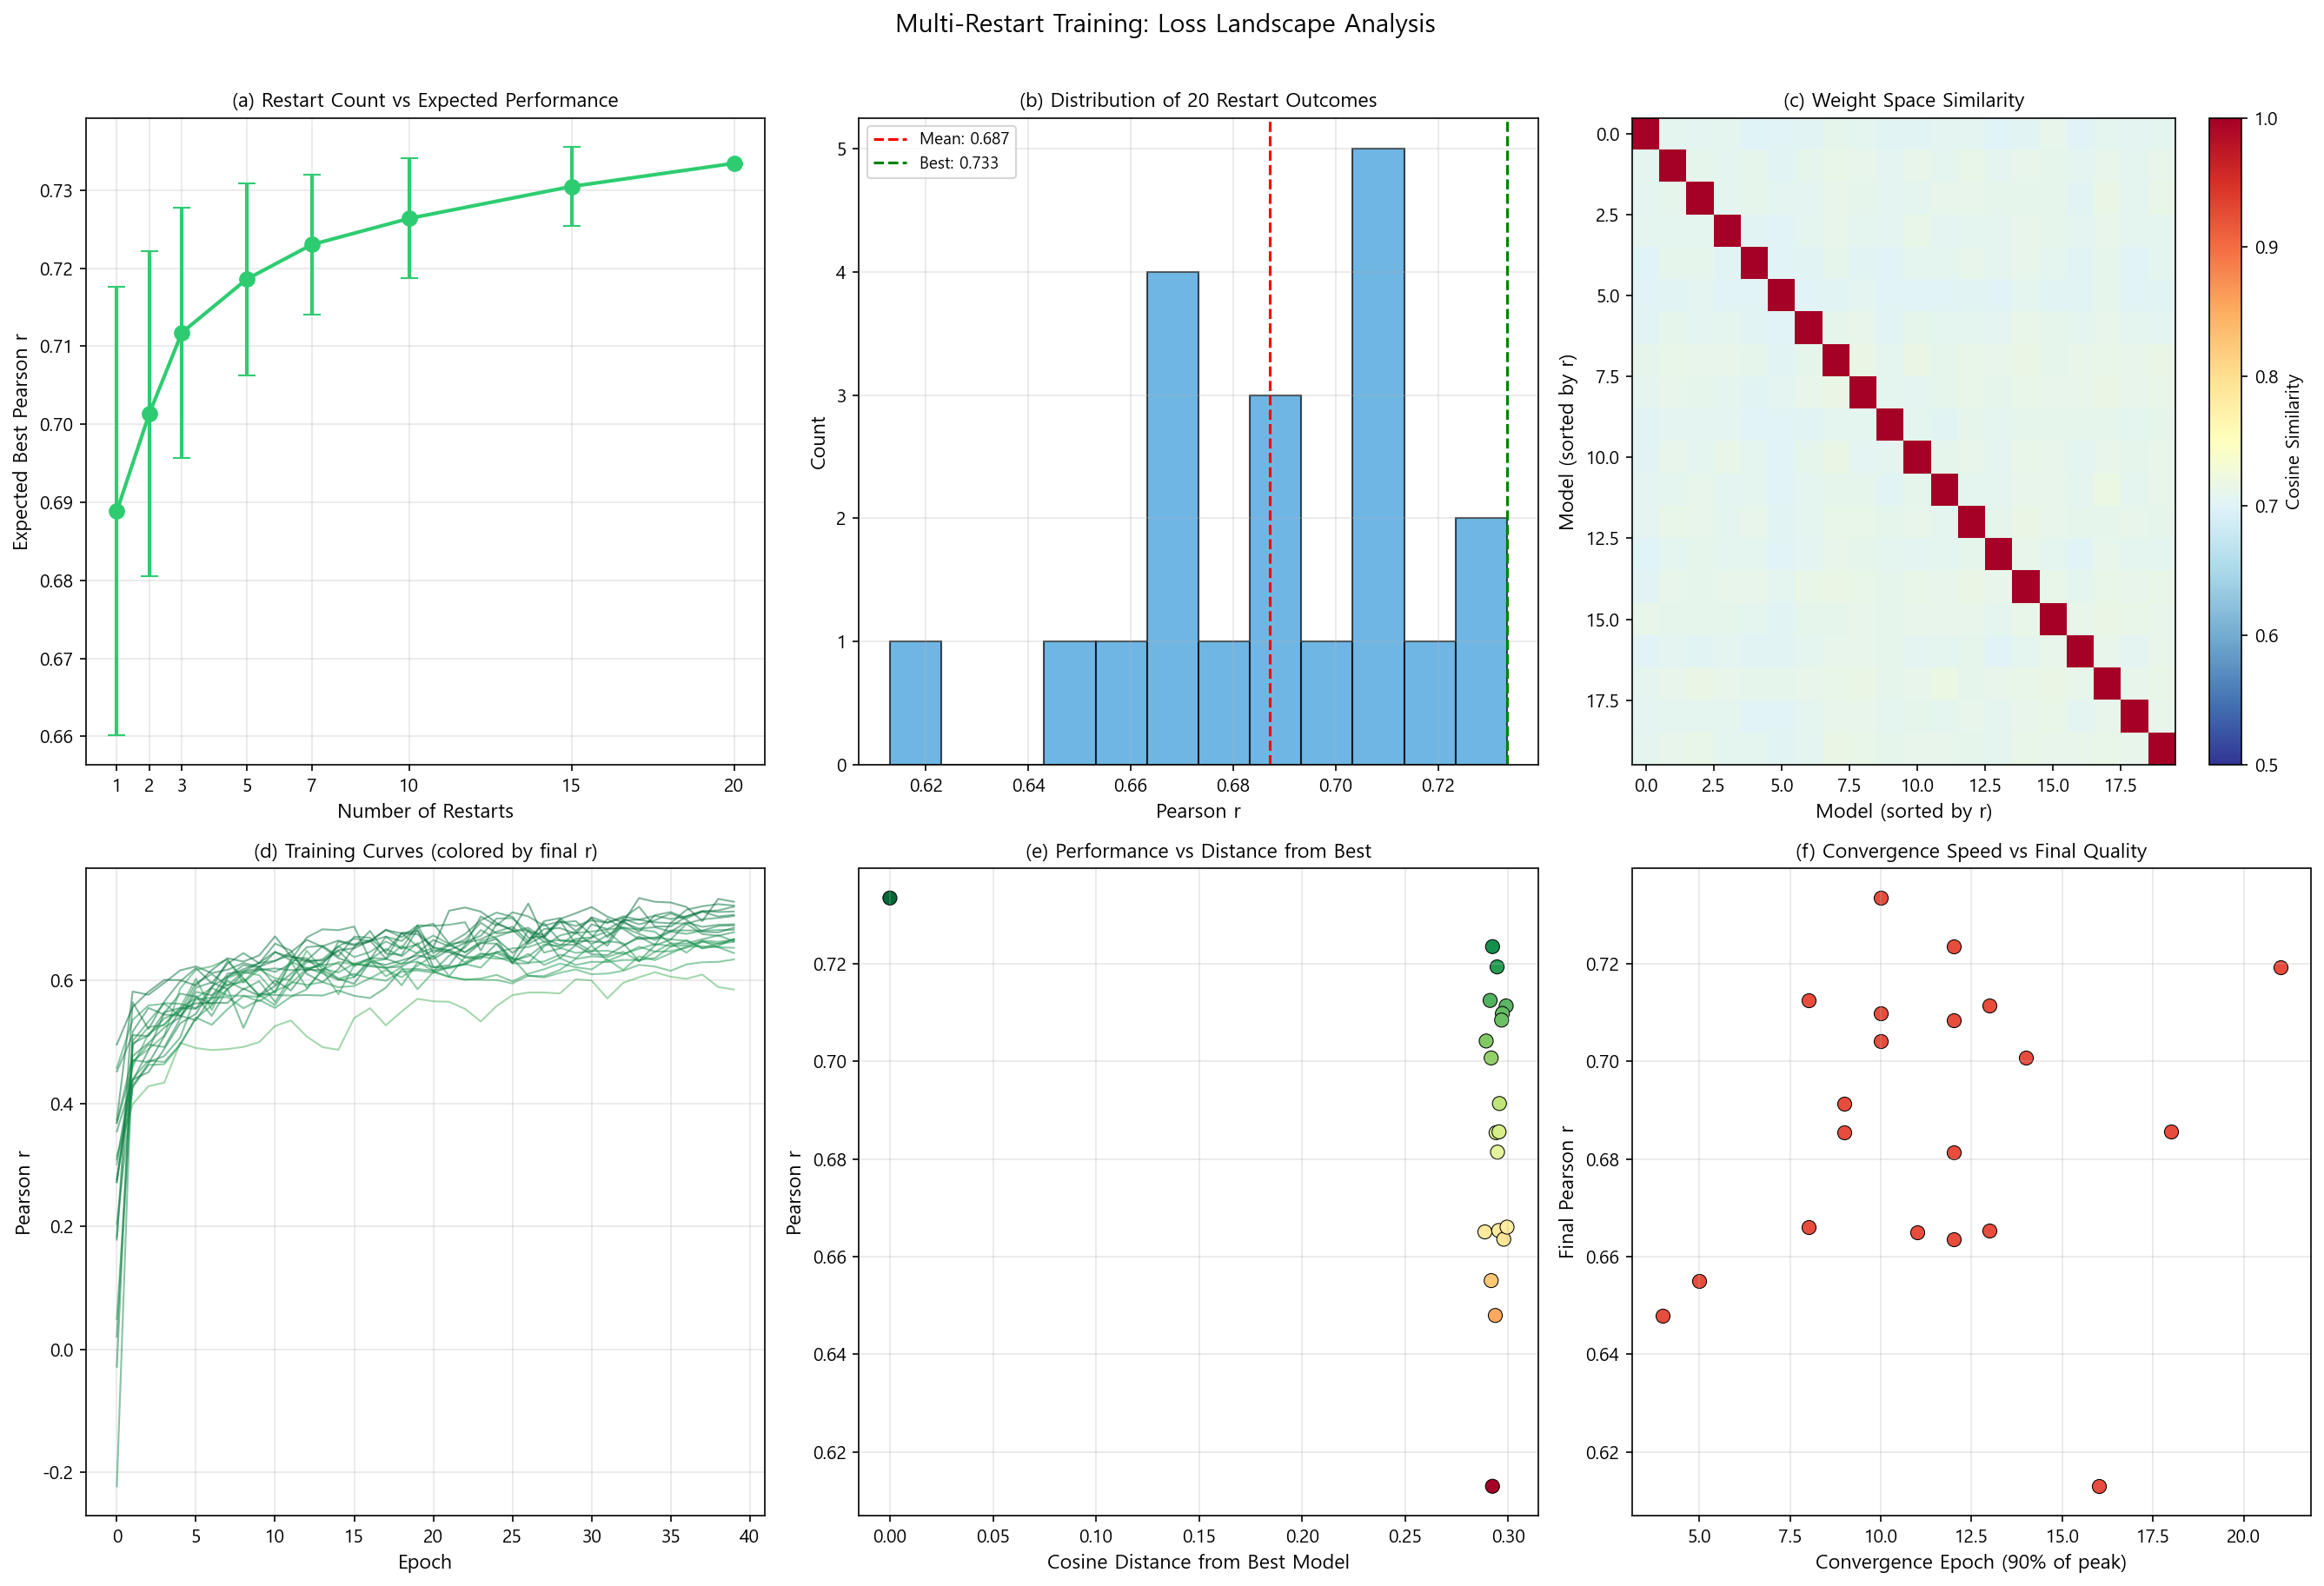
\includegraphics[width=0.95\textwidth]{figures/loss_landscape_analysis.png}
    \caption{Multi-restart loss landscape analysis. (a) Expected best $r$ vs restart count. (b) Distribution of 20 restart outcomes. (c) Weight-space cosine similarity heatmap. (d) Training curves colored by final $r$. (e) Performance vs cosine distance from best model. (f) Convergence speed vs final quality.}
    \label{fig:landscape}
\end{figure}

The 20 restarts produced final Pearson $r$ values with $\text{mean} = 0.687$, $\text{std} = 0.029$, ranging from 0.613 to 0.734. This variance provides direct evidence for the multi-modal nature of the loss landscape.

\begin{table}[H]
\centering
\caption{Expected best performance by restart count (100 Monte Carlo trials).}
\label{tab:restart}
\begin{tabular}{ccc}
\toprule
Restart Count & Expected Best $r$ & Std \\
\midrule
1 & 0.689 & 0.029 \\
3 & 0.712 & 0.016 \\
5 & 0.719 & 0.012 \\
10 & 0.726 & 0.008 \\
15 & 0.731 & 0.005 \\
20 & 0.734 & 0.000 \\
\bottomrule
\end{tabular}
\end{table}

The performance curve shows diminishing returns: $+0.023$ from 1 to 3 restarts, $+0.014$ from 3 to 10, and $+0.008$ from 10 to 20. This logarithmic scaling is consistent with order-statistics theory for sampling from a fixed distribution.

Weight-space analysis reveals mean pairwise cosine similarity of 0.709, indicating that converged models occupy distinct regions in weight space. The top-5 performing models show mean cosine similarity of 0.707, indistinguishable from the overall mean, confirming that high-quality solutions are scattered across the landscape rather than concentrated in a single basin.

These findings reframe multi-restart as an empirically justified response to a fundamentally multi-modal loss landscape, analogous to chaotic sensitivity in N-body systems where slight perturbations in initial conditions produce divergent trajectories.

\subsection{Small Data Regime Considerations}
With only 360 pairs, techniques designed for large datasets (contrastive learning, domain-shifted augmentation) are counterproductive. Simple architectures with multi-restart optimization outperform complex architectures with sophisticated training.

\section{Conclusion}

We presented Universe Multi Neural network (UMN), a differentiable N-body gravitational simulation architecture for olfactory mixture similarity prediction. UMN achieves $r = 0.780$ on the Snitz dataset using 5-seed $\times$ 5-fold cross-validation without manual feature engineering. Key findings: (1) the physics engine architecture is near-optimal in its simplest form, (2) multi-restart training is the most effective strategy for the multi-modal loss landscape, (3) contrastive learning and physics-based losses are counterproductive in small-data regimes, and (4) learned physical quantities show partial chemical interpretability through correlations with LogP and HBA.

Limitations include the small dataset size (360 pairs), the absence of identical-protocol comparison with Snitz et al. (2013), and the weak effect sizes ($|r| < 0.15$) in the interpretability analysis. Future directions include larger datasets, deeper interpretability via attention on learned trajectories, simulation-GNN ensembles, and concentration-aware models.

\begin{thebibliography}{12}

\bibitem[Bushdid et al.(2014)]{bushdid2014}
Bushdid, C., Magnasco, M.~O., Vosshall, L.~B., and Keller, A.
\newblock Humans can discriminate more than 1 trillion olfactory stimuli.
\newblock \textit{Science}, 343(6177):1370--1372, 2014.

\bibitem[Chen et al.(2018)]{chen2018}
Chen, R.~T.~Q., Rubanova, Y., Bettencourt, J., and Duvenaud, D.
\newblock Neural ordinary differential equations.
\newblock In \textit{NeurIPS}, 31:6571--6583, 2018.

\bibitem[Gilmer et al.(2017)]{gilmer2017}
Gilmer, J., Schoenholz, S.~S., Riley, P.~F., Vinyals, O., and Dahl, G.~E.
\newblock Neural message passing for quantum chemistry.
\newblock In \textit{ICML}, pp.~1263--1272, 2017.

\bibitem[Greydanus et al.(2019)]{greydanus2019}
Greydanus, S., Dzamba, M., and Yosinski, J.
\newblock Hamiltonian neural networks.
\newblock In \textit{NeurIPS}, 32:8026--8037, 2019.

\bibitem[Keller et al.(2017)]{keller2017}
Keller, A., Gerkin, R.~C., Guan, Y., et al.
\newblock Predicting human olfactory perception from chemical features of odor molecules.
\newblock \textit{Science}, 355(6327):820--826, 2017.

\bibitem[Kipf et al.(2018)]{kipf2018}
Kipf, T., Fetaya, E., Wang, K.-C., Welling, M., and Zemel, R.
\newblock Neural relational inference for interacting systems.
\newblock In \textit{ICML}, pp.~2688--2697, 2018.

\bibitem[Lee et al.(2023)]{lee2023}
Lee, B.~K., Mayhew, E.~J., Sanchez-Lengeling, B., et al.
\newblock A principal odor map unifies diverse tasks in human olfaction.
\newblock \textit{Science}, 381(6661):999--1006, 2023.

\bibitem[Raissi et al.(2019)]{raissi2019}
Raissi, M., Perdikaris, P., and Karniadakis, G.~E.
\newblock Physics-informed neural networks.
\newblock \textit{Journal of Computational Physics}, 378:686--707, 2019.

\bibitem[Ravia et al.(2020)]{ravia2020}
Ravia, A., Snitz, K., Honigstein, D., et al.
\newblock A measure of smell enables the creation of olfactory metamers.
\newblock \textit{Nature}, 588(7836):118--123, 2020.

\bibitem[Rogers and Hahn(2010)]{rogers2010}
Rogers, D. and Hahn, M.
\newblock Extended-connectivity fingerprints.
\newblock \textit{J.~Chem.~Inf.~Model.}, 50(5):742--754, 2010.

\bibitem[Snitz et al.(2013)]{snitz2013}
Snitz, K., Yablonka, A., Weiss, T., Frumin, I., Khan, R.~M., and Sobel, N.
\newblock Predicting odor perceptual similarity from odor structure.
\newblock \textit{PLoS Computational Biology}, 9(9):e1003184, 2013.

\bibitem[Yang et al.(2019)]{yang2019}
Yang, K., Swanson, K., Jin, W., et al.
\newblock Analyzing learned molecular representations for property prediction.
\newblock \textit{J.~Chem.~Inf.~Model.}, 59(8):3370--3388, 2019.

\end{thebibliography}

\end{document}
